% !TEX root =  ../ms.tex

\section{Joint Model}
\label{sec : joint_model}
Our goal is to check if SCr and PCR both, are useful to predict graft failure. To this end, we model the two longitudinal outcomes and graft failure together using joint models (JMs) for time to event and longitudinal data \citep{tsiatis2004joint,rizopoulos2012joint}. In this model we use log transformed values of both SCr and PCR \citep{fournier2016joint}. More specifically, we model the impact of log(SCr) value and log(SCr) velocity, log(PCR) value and log(PCR) velocity, and transplantation characteristics on the hazard of graft failure. In this regard, the JM consists of a multivariate longitudinal sub-model to model the evolution of SCr and PCR and a relative risk sub-model to model the impact of transplantation characteristics and biomarkers on the hazard of graft failure. The longitudinal evolution of the two outcomes over time is modeled flexibly using B-splines. The model formulation for PCR outcome is as follows (for SCr outcome it is same):

\begin{equation}
\label{eq : long_model_prias}
\begin{aligned}
\log \mbox{PCR}(t) &= \beta_0 + \beta_1 \mbox{rec\_age} + \beta_2 \mbox{d\_age} + \beta_3 \mbox{d\_bmi} + \beta_4 \mbox{rec\_bmi} + \beta_5 \mbox{cit}\\
&+ \beta_6 \mbox{hla} + \beta_7 \mbox{pra}+ \beta_8 \mbox{dial\_days} + \beta_9 \mbox{ah\_nr} + \beta_{10} \mbox{rec\_gender} + \beta_{11} \mbox{d\_gender} \\
&+ \beta_{12} \mbox{dgf} + \beta_{13} \mbox{prev\_tp} + \beta_{14} \mbox{dm} + \beta_{15} \mbox{hvdis}+ \beta_{16} \mbox{d\_cadaveric}\\
&+\sum_{k=1}^4 \beta_{k+16} B_k(t,\mathcal{K}) +  b_{i0} + \sum_{k=1}^4 b_{ik} B_k(t,\mathcal{K}) + 
\varepsilon_i(t),
\end{aligned}
\end{equation}
where $B_k(t, \mathcal{K})$ denotes the $k$-th basis function of a B-spline with three internal knots at $\mathcal{K} =\{0.082, 0.219, 1\}$ (30 and 80 days recommended by the clinicians) years, and boundary knots at 0.039 and 6 years (minimum and 0.95 quantile of the time of measurements two outcomes). The quantitative transplantation characteristics are standardized to avoid convergence issues in parameter estimation. For the relative risk sub-model the hazard function we fit is given by:
\begin{equation}
\label{eq : hazard_prias}
h_i(t) = h_0(t) \exp\big\{\gamma_1 \mbox{prev\_tp} + \gamma_2 \mbox{hla}  + \gamma_3 \mbox{cit} + \gamma_4 \mbox{dial\_days} + \alpha_1 m_{i1}(t) + \alpha_2 m'_{i1}(t)\big\}.
\end{equation}
where $\alpha_1$ and $\alpha_2$ are measures of strength of the association between hazard of graft failure and $\log \mbox{PCR}$ value $m_{i1}(t)$ and $\log \mbox{PCR}$ velocity $m'_{i1}(t)$, respectively.

The parameters of the JM are estimated using the R package \textbf{JMbayes} \citep{rizopoulosJMbayes}, which uses the Bayesian methodology to estimate the model parameters (section B, supplementary material). Out of 239 patients, we use the data of only those 238 patients for whom both PCR and SCr data is available. The parameter estimates for the longitudinal sub-model for SCr and PCR are provided in Table \ref{tab : creatinine_long} and Table \ref{tab : pcr_long}, respectively. The effect of transplantation characteristics on both outcomes is small and ignorable, and hence not discussed in detail. Since the quantitative variables are standardized, the effect sizes correspond to one standard deviation increase in the corresponding variable. To avoid the tricky interpretation of variables corresponding to evolution over time, instead the evolution of SCr and PCR over time is depicted in Figure \ref{fig : creatinine_evolution}, and Figure \ref{fig : pcr_evolution}, respectively.
@Hessel: We have to explain why the creatinine levels dip. 

\begin{table}[!htb]
\begin{center}
\caption{Parameter estimates for the longitudinal model for SCr.}
\label{tab : creatinine_long}
\begin{tabular}{lrrrrr}
\Hline
Variable                                                                         & Mean   & Std. Dev & 2.5\%  & 97.5\% & P              \\
\hline
Intercept                                                                      & 5.226  & 0.080    & 5.064  & 5.378  & \textless0.000 \\
Receiver age                                                                   & -0.063 & 0.022    & -0.107 & -0.019 & 0.010          \\
Donor age                                                                          & 0.083  & 0.020    & 0.045  & 0.119  & \textless0.000 \\
Donor BMI                                                                          & -0.011 & 0.021    & -0.054 & 0.028  & 0.612          \\
Receiver BMI                                                                         & 0.018  & 0.023    & -0.025 & 0.060  & 0.420          \\
\#HLA mismatches between donor and recipient                                                                         & 0.020  & 0.022    & -0.022 & 0.065  & 0.342          \\
Panel reactive antibody percentage                                                                          & 0.048  & 0.027    & -0.008 & 0.100  & 0.082          \\
\#Anti-hypertensive medicaments                                                                           & 0.040  & 0.020    & 0.001  & 0.080  & 0.048          \\
Cold ischemia time                                                                         & 0.029  & 0.035    & -0.039 & 0.102  & 0.390          \\
\#Days on dialysis before transplant                                                                   & 0.015  & 0.029    & -0.042 & 0.071  & 0.580          \\
Receiver gender: Male                                                                     & 0.197  & 0.042    & 0.111  & 0.276  & \textless0.000 \\
Previous transplant: Yes                                                                & 0.016  & 0.064    & -0.115 & 0.141  & 0.786          \\
Donor gender: Male                                                                      & 0.053  & 0.042    & -0.027 & 0.136  & 0.198          \\
Delayed graft function: Yes                                                                       & 0.118  & 0.049    & 0.025  & 0.216  & 0.006          \\
Diabetes Mellitus: Yes                                                                        & -0.103 & 0.059    & -0.217 & 0.012  & 0.076          \\
Cardiovascular events before transplantation: Yes                                                                     & -0.047 & 0.043    & -0.129 & 0.044  & 0.272          \\
Deceased donor: Yes                                                                 & 0.163  & 0.082    & 0.004  & 0.313  & 0.044          \\
Spline: visit time [0.039, 0.082] years & -0.440 & 0.041    & -0.517 & -0.358 & \textless0.000 \\
Spline: visit time [0.082, 0.219] years & -0.182 & 0.053    & -0.284 & -0.081 & \textless0.000 \\
Spline: visit time [0.219, 1] years & -0.545 & 0.081    & -0.712 & -0.395 & \textless0.000 \\
Spline: visit time [1, 6] years & 0.007  & 0.083    & -0.155 & 0.176  & 0.946          \\
$\sigma$                                                                            & 0.190  & 0.001    & 0.187  & 0.192  & \\
\hline
\end{tabular}
\end{center}
\end{table}

\begin{table}[!htb]
\begin{center}
\caption{Parameter estimates for the longitudinal model for PCR.}
\label{tab : pcr_long}
\begin{tabular}{lrrrrr}
\Hline
              Variable                                                                   & Mean   & Std. Dev & 2.5\%  & 97.5\% & P              \\
              \hline
Intercept                                                                      & 3.731  & 0.179    & 3.398  & 4.083  & \textless0.000 \\
Receiver age                                                                   & 0.030  & 0.052    & -0.066 & 0.138  & 0.604          \\
Donor age                                                                          & 0.209  & 0.047    & 0.118  & 0.301  & \textless0.000 \\
Donor BMI                                                                          & -0.019 & 0.051    & -0.121 & 0.084  & 0.716          \\
Receiver BMI                                                                         & -0.116 & 0.050    & -0.219 & -0.021 & 0.014          \\
\#HLA mismatches between donor and recipient                                                                         & -0.013 & 0.049    & -0.112 & 0.086  & 0.776          \\
Panel reactive antibody percentage                                                                          & 0.047  & 0.061    & -0.066 & 0.166  & 0.446          \\
\#Anti-hypertensive medicaments                                                                           & 0.056  & 0.047    & -0.03  & 0.147  & 0.208          \\
Cold ischemia time                                                                         & 0.062  & 0.082    & -0.097 & 0.211  & 0.468          \\
\#Days on dialysis before transplant                                                                   & 0.006  & 0.066    & -0.120 & 0.134  & 0.952          \\
Receiver gender: Male                                                                     & -0.026 & 0.094    & -0.207 & 0.166  & 0.798          \\
Previous transplant: Yes                                                                & 0.035  & 0.149    & -0.241 & 0.332  & 0.816          \\
Donor gender: Male                                                                      & 0.114  & 0.096    & -0.079 & 0.303  & 0.228          \\
Delayed graft function: Yes                                                                       & 0.043  & 0.118    & -0.174 & 0.275  & 0.740          \\
Diabetes Mellitus: Yes                                                                        & 0.153  & 0.135    & -0.124 & 0.396  & 0.256          \\
Cardiovascular events before transplantation: Yes                                                                     & -0.016 & 0.106    & -0.221 & 0.199  & 0.890          \\
Deceased donor: Yes                                                                  & 0.144  & 0.193    & -0.246 & 0.509  & 0.462          \\
Spline: visit time [0.039, 0.082] years & -0.821 & 0.090    & -0.989 & -0.638 & \textless0.000 \\
Spline: visit time [0.082, 0.219] years & -0.578 & 0.131    & -0.838 & -0.304 & \textless0.000 \\
Spline: visit time [0.219, 1] years & -0.898 & 0.160    & -1.218 & -0.587 & \textless0.000 \\
Spline: visit time [1, 6] years & 0.460  & 0.234    & 0.015  & 0.927  & 0.036          \\
$\sigma$                                                                            & 0.479  & 0.004    & 0.472  & 0.486  & \\
\hline
\end{tabular}
\end{center}
\end{table}

\begin{figure}[!htb]
\centerline{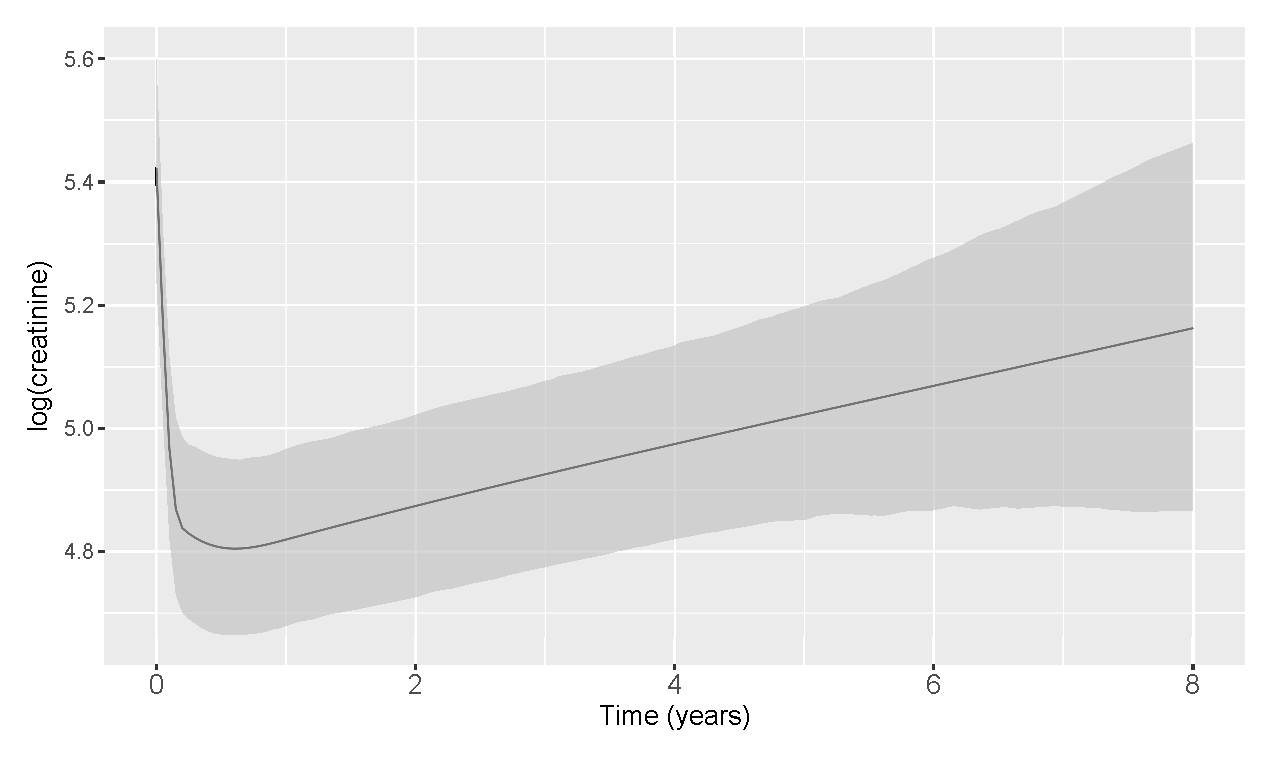
\includegraphics[width=\columnwidth]{images/creatinine.eps}}
\caption{Fitted longitudinal evolution of SCr and 95\% credible interval for a patient with the  transplantation characteristics described in Table \ref{tab : baseline_characteristics}.}
\label{fig : creatinine_evolution}
\end{figure}

\begin{figure}[!htb]
\centerline{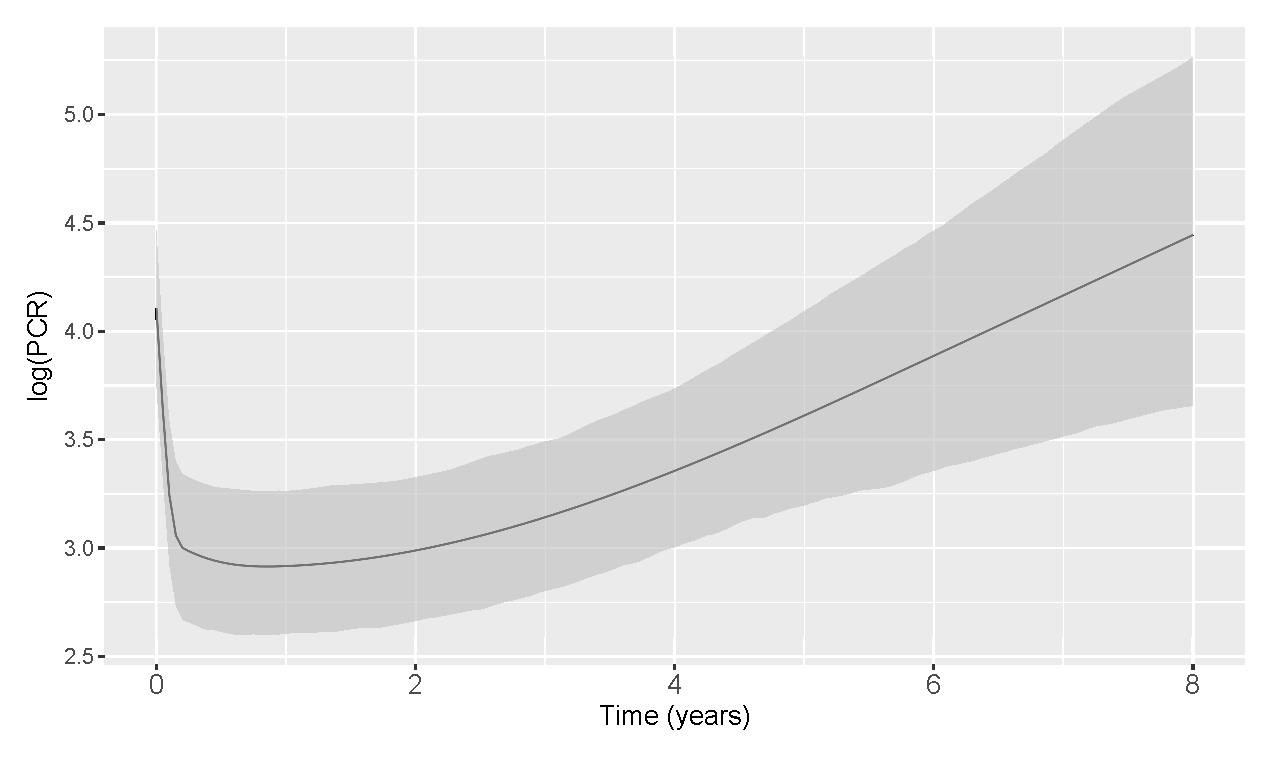
\includegraphics[width=\columnwidth]{images/pcr.eps}}
\caption{Fitted longitudinal evolution of PCR and 95\% credible interval for a patient with the  transplantation characteristics described in Table \ref{tab : baseline_characteristics}.}
\label{fig : pcr_evolution}
\end{figure}

The parameter estimates for the relative risk sub-model are provided in Table \ref{tab : relative_risk}. Since the quantitative variables are standardized, the effect sizes correspond to one standard deviation increase in the corresponding variable. We found that the $\log \mbox{SCr}$  levels are strongly associated with the hazard of GR. More specifically, for a given patient, if the SCr levels become twice and the remaining variables in the relative risk model remain the same, the hazard of graft failure increases three fold. $\log \mbox{PCR}$ levels and velocity are not strongly associated with hazard of GR. To further verify if they are required in the model in presence of both $\log \mbox{SCr}$ levels and velocity, we fitted two more JMs. In the first JM we modeled the association between $\log \mbox{SCr}$ levels and velocity and hazard of graft failure. In the second JM we modeled the association between $\log \mbox{PCR}$ levels and velocity and hazard of graft failure. We then calculated time dependent AUC, that is, area under the curve \citep{landmarking2017,rizopoulosJMbayes} values for all of the three JMs. The time dependent AUC were calculated periodically at an interval of 6 months. The first AUC was calculated at 6 months since transplantation and the last AUC was calculated at 3 years since transplantation. The resulting AUC values are plotted in Figure \ref{fig : auc_curve} and listed in Table \ref{tab : auc}. It can be seen that the model with both longitudinal outcomes performs the same as the model with only creatinine, to discriminate between patients who obtain graft failure versus others. Hence modeling PCR may not be necessary.

\begin{table}[!htb]
\begin{center}
\caption{Relative risk sub-model estimates for mean and 95\% credible interval.}
\label{tab : relative_risk}
\begin{tabular}{lrrrrr}
\Hline
Variable               & Mean   & Std. Dev & 2.5\%  & 97.5\% & P              \\
\hline
Previous transplant: Yes      & 0.305  & 0.339    & -0.099 & 0.986  & 0.352          \\
\#HLA mismatches between donor and recipient                & 0.048  & 0.093    & -0.114 & 0.269  & 0.620          \\
Cold ischemia time                & -0.051 & 0.105    & -0.277 & 0.133  & 0.644          \\
\#Days on dialysis before transplant         & -0.013 & 0.102    & -0.251 & 0.178  & 0.934          \\
$\log \mbox{PCR}$        & 0.145  & 0.125    & -0.056 & 0.431  & 0.188          \\
Slope($\log \mbox{PCR}$)        & 0.021  & 0.058    & -0.076 & 0.145  & 0.828          \\
$\log \mbox{SCr}$ & 1.599  & 0.241    & 1.067  & 2.063  & \textless0.000 \\
Slope($\log \mbox{SCr}$)  & 0.203  & 0.123    & -0.017 & 0.443  & 0.082  \\
\hline
\end{tabular}
\end{center}
\end{table}

\begin{figure}[!htb]
\centerline{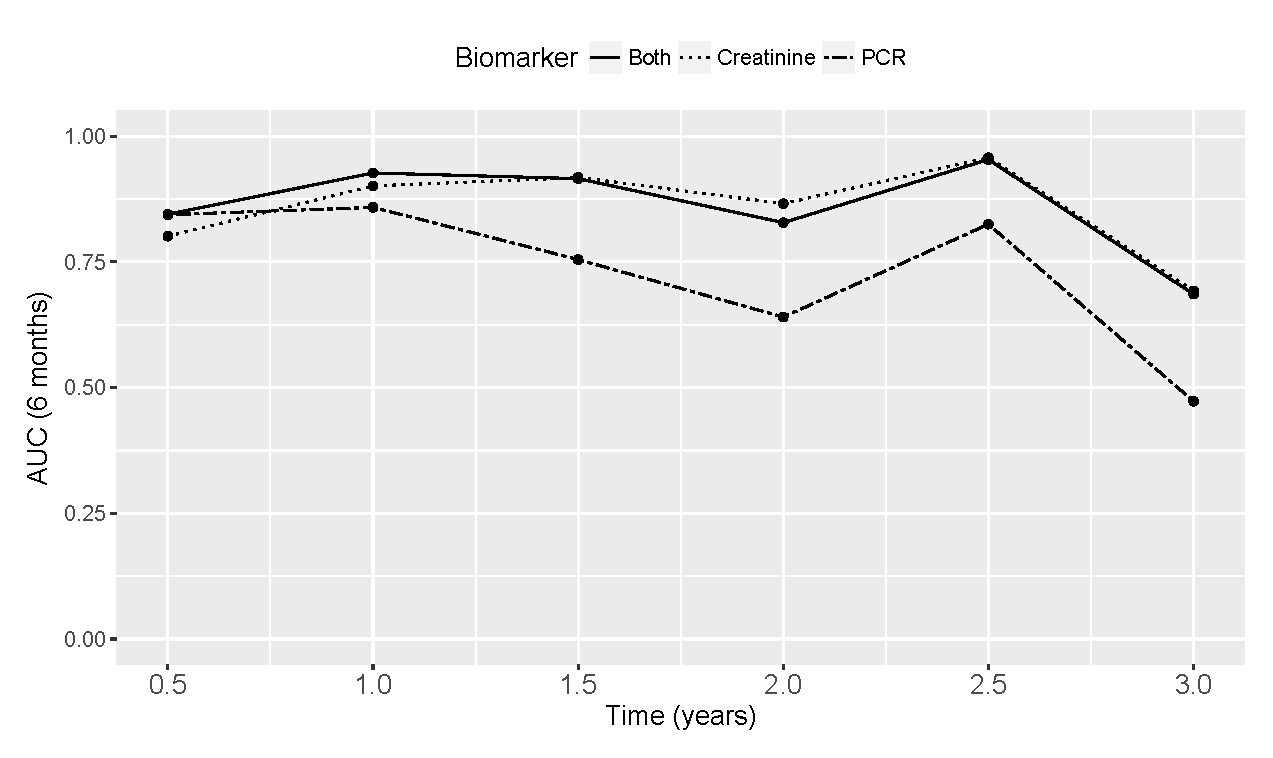
\includegraphics[width=\columnwidth]{images/auc.eps}}
\caption{Area under curve characteristics for the JMs fitted to the kidney transplant data set.}
\label{fig : auc_curve}
\end{figure}

\begin{table}[!htb]
\begin{center}
\caption{Area under curve characteristics for the JMs fitted to the kidney transplant data set.}
\label{tab : auc}
\begin{tabular}{lrrrrrr}
\Hline
Biomarkers               & Year 0.5   & Year 1 & Year 1.5  & Year 2 & Year 2.5 & Year 3 \\
\hline
Both SCr and PCR & 0.845 & 0.927 & 0.915 & 0.828 & 0.953 & 0.686\\
Only SCr & 0.801 & 0.901 & 0.918 & 0.866 & 0.957 & 0.692\\
Only PCR & 0.844 & 0.858 & 0.755 & 0.640 & 0.825 & 0.473\\
\hline
\end{tabular}
\end{center}
\end{table}